\documentclass[12pt]{kiarticle}
\graphicspath{{pictures/}}
\DeclareGraphicsExtensions{.pdf,.png,.jpg,.eps}
%%%
\pagestyle{fancy}
\fancyhf{}
%\renewcommand{\headrulewidth}{ 0.1mm }
\renewcommand{\footrulewidth}{ .0em }
\fancyfoot[C]{\texttt{\textemdash~\thepage~\textemdash}}
\fancyhead[L]{Лабораторная работа № 4.5.2 \hfil}
\fancyhead[R]{\hfil Иванов Кирилл, 625 группа }
\usepackage{multirow} % Слияние строк в таблице
\newcommand
{\un}[1]
{\ensuremath{\text{#1}}}
\newcommand{\eds}{\ensuremath{ \mathscr{E}}}
\usepackage{tikz}
%%% Работа с таблицами
\usepackage{array,tabularx,tabulary,booktabs} % Дополнительная работа с таблицами
\usepackage{longtable}  % Длинные таблицы
\usepackage{multirow} % Слияние строк в таблице

\begin{document}
	
	\begin{titlepage}
	\begin{center}
		\large 	Московский физико-технический институт \\
		(государственный университет) \\
		Факультет общей и прикладной физики \\
		\vspace{0.2cm}
		
		\vspace{4.5cm}
		Лабораторная работа № 4.5.2 \\ \vspace{0.2cm}
		\large (Общая физика: оптика) \\ \vspace{0.2cm}
		\LARGE \textbf{Интерференция лазерного излучения}
	\end{center}
	\vspace{2.3cm} \large
	
	\begin{center}
		Работу выполнил: \\
		Иванов Кирилл,
		625 группа
		\vspace{10mm}		
		
	\end{center}
	
	\begin{center} \vspace{60mm}
		г. Долгопрудный \\
		2018 год
	\end{center}
\end{titlepage}
	
	\paragraph*{Цель работы:} исследование видности интерференционной картины излучения гелий-неонового лазера и определение длины когерентности излучения.
	
	\paragraph*{Оборудование:}  $Не-Nе$-лазер, интерферометр Майкельсона с подвижным зеркалом, фотодиод с усилителем, осциллограф, поляроид, линейка.
	
	\section{Теоретическое введение}
	
	Важный параметр интерференционной картины --- ее видимость:
	
	\begin{equation}\label{V0}
	V = \dfrac{I_{max} - I_{min}}{I_{max} + I_{min}}
	\end{equation}
	
	Удобно представлять видимость в виде произведения функций различных параметров установки/системы:
	
	\begin{equation}\label{VVV}
	V = V_1 V_2 V_3
	\end{equation}
	
	Рассмотрим эти функции подробнее. Первая из них отвечает за отношение интенсивностей интерферирующих волн:
	
	\begin{equation}\label{V1}
	V_1 = \dfrac{2\sqrt{\delta}}{1 + \delta}, \quad \delta = \dfrac{B_m^2}{A_m^2}
	\end{equation}
	
	
	Здесь $ A_m, B_m $ --- амплитуды волн. Вторая функция учитывает влияние разности хода и спектрального состава волн:
	
	
	\begin{equation}\label{}
	\gamma_2 = \dfrac{\sum\limits_n A_n^2 \cos{\dfrac{2\pi \Delta \nu n l}{c}}}{\sum\limits_n A_n^2} \sim e^{-(\pi \Delta F l /c^2)}
	\end{equation}
	
		\begin{wrapfigure}{l}{0.35\linewidth} 
		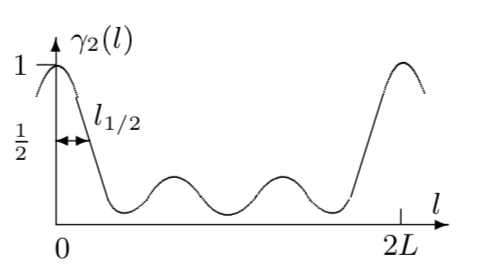
\includegraphics[width=\linewidth]{v2.png}
		\caption{Качественный график $ V_2 $}
		\label{V2graf}
	\end{wrapfigure}
	
	
	Здесь $ l $ --- разность хода, $ \Delta\nu $ --- спектральный состав излучения, $ A_n^2 $ --- интенсивность мод. Оценка приведена из перехода к непрерывному пределу. На графике (рис.\ref{V2graf}) показан вид $ V_2(l) $, позволяющий получить расстояние $ L $ между зеркалами резонатора и межмодовое расстояние $ \Delta \nu $. Величина $ l_{1/2} $  позволяет оценить диапазон частот $ \Delta F $.
	Формулы связи межмодового расстояния и длины $ L $, а также $ l_{1/2} \; и \; \Delta F $ таковы:
	
	\begin{equation}\label{dnu}
	\Delta \nu = \dfrac{c}{2L}, \quad l_{1/2} \approx \dfrac{0,26 c}{\Delta F}
	\end{equation}
	
	Последняя функция --- зависимость от угла поляризации $ \alpha $:
	
	\begin{equation}\label{}
	V_3 = |\cos{\alpha}|
	\end{equation}
	
	\section{Экспериментальная установка}
	
	\subsection{Описание установки}
	
	Для получения интерференционной картины используется интерферометр Майкельсона, смонтированный на вертикально стоящей массивной металлической плите. Схема установки приведена на рисунке.
	
\begin{figure}[h!]
		\centering
		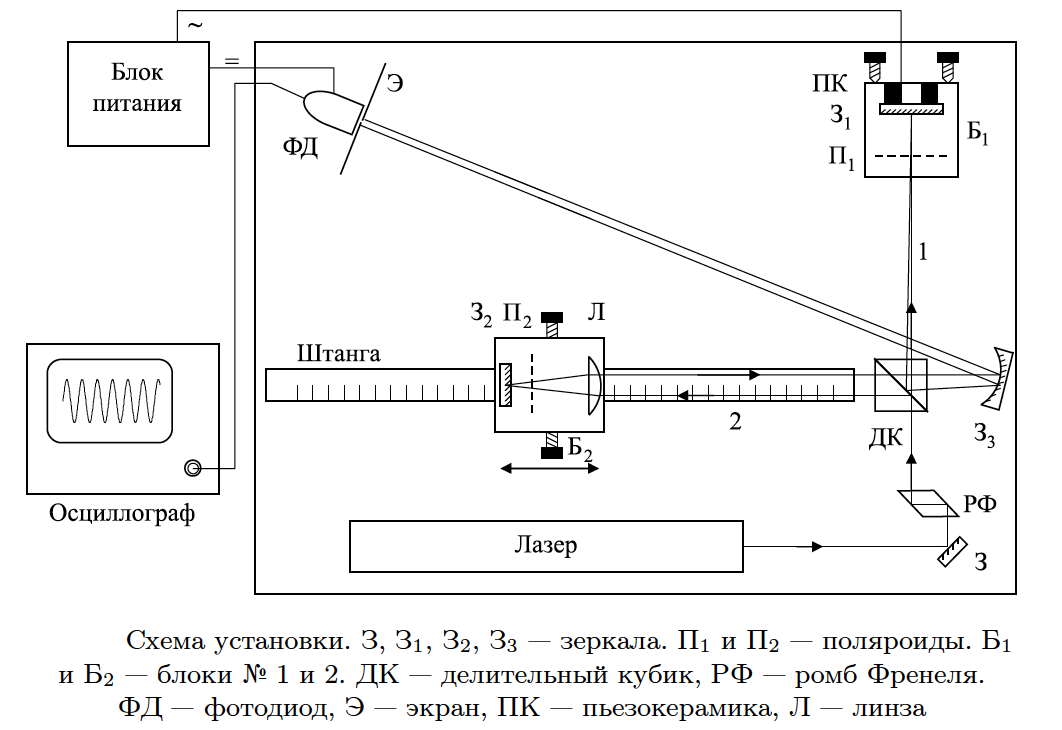
\includegraphics[width=\linewidth]{lab.png}
%		\caption{Экспериментальная установка}
		\label{lab}
\end{figure}

Источником света служит гелий-неоновый лазер (средняя длина
волны $ \lambda_0 = 632,8 $ нм). Пучок лазерного излучения отражается от зеркала З и проходит призму полного внутреннего отражения РФ (ромб Френеля), которая превращает линейную поляризацию излучения в круговую. Если в установке используется лазер, излучающий неполяризованный свет, то ромб Френеля не нужен, но он и не мешает выполнению
работы. Далее лазерное излучение делится диагональной плоскостью
делительного кубика ДК на два пучка.

Пучок 1 проходит поляроид $ П_1, $ отражается под небольшим углом
от зеркала $ З_1 $, снова проходит поляроид $ П_1 $ и, частично отражаясь от
диагональной плоскости делительного кубика, выходит из интерферометра, попадает на зеркало $ З_3 $ и далее на фотодиод ФД. Зеркало $ З_1 $
наклеено на пьезокерамику ПК, которая может осуществлять малые колебания зеркала вдоль направления распространения падающего пуч-
ка. Поляроид и зеркало с пьезокерамикой собраны в единый блок $ Б_1 $,
который крепится к вертикально стоящей плите. В блоке $ Б_1 $ имеются
юстировочные винты, которые позволяют регулировать угол наклона
зеркала $ З_1 $. В установке предусмотрена возможность вращения поляро-
ида $ П_1 $. Угол поворота отсчитывается по шкале, нанесённой на оправу
поляроида.
Пучок 2 проходит линзу Л, поляроид $ П_2 $, отражается от зеркала $ З_2 $,
снова проходит поляроид $ П_2 $, линзу Л и делительный кубик, выходит из
интерферометра, попадает на зеркало $ З_3 $ и далее на фотодиод ФД. Та-
ким образом, от зеркала $ З_3 $ под небольшим углом друг к другу идут на
фотодиод два пучка, прошедшие разные плечи интерферометра. Меж-
ду ними происходит интерференция и образуются интерференционные
полосы. Линза Л, поляроид $ П_2 $ и зеркало $ З_2 $ собраны в единый блок $ Б_2 $.

Зеркало $ З_2 $ установлено в фокальной плоскости линзы Л. Это сделано
для того, чтобы падающий и выходящий из блока $ Б_2 $ пучки всегда были
параллельны друг другу. Блок $ Б_2 $ может перемещаться вдоль пучка 2
по штанге, жёстко связанной с плитой интерферометра. Длина штанги
90 см. В установке предусмотрена возможность небольшого поперечно-
го перемещения блока $ Б_2 $, что позволяет регулировать расстояние меж-
ду падающим и выходящим из блока пучками. При измерениях блок
Б2 крепится к штанге при помощи двух винтов. Вдоль штанги нанесены деления через один сантиметр. При перемещении блока $ Б_2 $ вдоль
штанги на величину $ x_1 $ геометрическая разность хода между пучками
1 и 2 изменяется на величину $ l = 2x_1 $.

Сферическое зеркало $ З_3 $ с небольшим фокусным расстоянием увеличивает картину интерференционных полос и позволяет наблюдать её
на экране Э, расположенном в плоскости входного окна фотодиода.
Свет попадает на фотодиод ФД через узкую щель в центре экрана.
Щель ориентируется параллельно интерференционным полосам. Ширина щели меньше расстояния между полосами. Сигнал фотодиода усиливается и подаётся на вход осциллографа. Для питания усилителя
сигнала фотодиода и управления пьезокерамикой используется блок
питания БП.

На пьезокерамику подаётся напряжение с частотой 50 Гц. При этом
её длина изменяется с частотой 100 Гц. Величина удлинения зависит от
приложенного напряжения и регулируется ручкой "<Качание"> на блоке
питания. Обычно удлинение составляет несколько длин волн света. На
эту величину перемещается вдоль пучка 1 зеркало $ З_1 $. Интерференционная картина смещается на ширину полосы (одно колебание на экране осциллографа), если зеркало $ З_1 $ смещается на $ \lambda_0 /2 \sim 0,3 $ мкм. При
измерениях через входную щель фотодиода последовательно проходит
несколько полос интерференционной картины, а на экране осциллографа наблюдаются колебания с изменяющимся периодом.

\subsection{Методика измерения}

\begin{wrapfigure}{l}{0.35\linewidth} 
	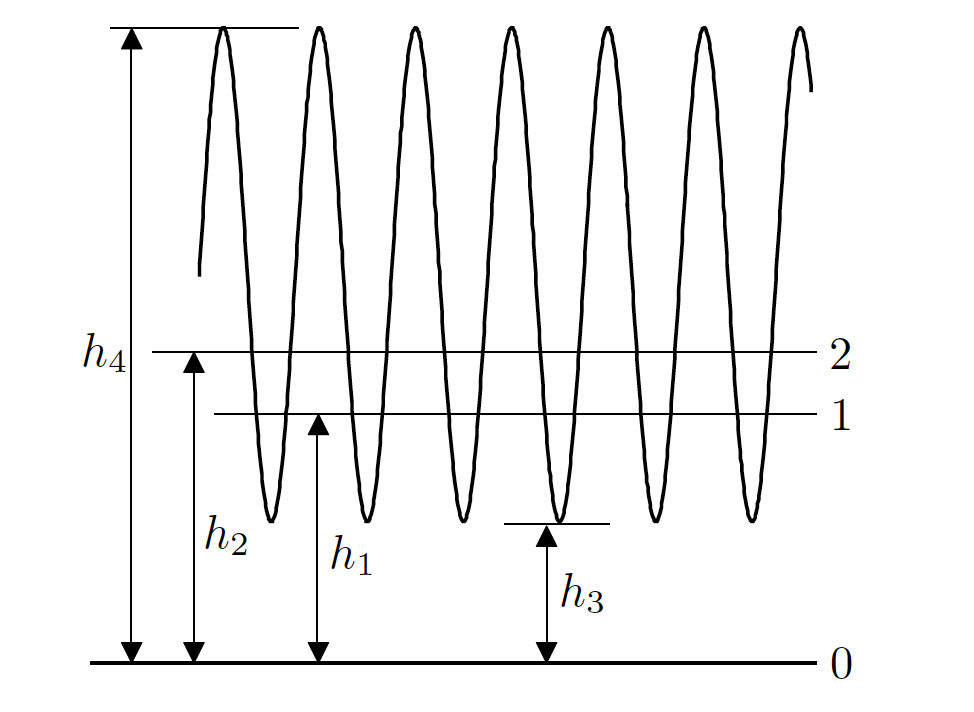
\includegraphics[width=\linewidth]{os}
	\caption{Сигнал фотодиода на осциллографе}
	\label{}
\end{wrapfigure}

	Осциллограф мы используем для нахождения следующих вели-
чин: фоновой засветки (линия 0 --- перекрыты оба пучка 1 и 2); интенсивность света каждого из пучков (линии 1 или 2 --- перекрыт пучок
2 или 1); максимума и минимума интенсивности интерференционной
картины (открыты оба пучка). При этом параметр $ \delta $ из \eqref{V1},  определяется отношением

\begin{equation}\label{delta}
\delta = \dfrac{h_1}{h_2}
\end{equation}

Понятно, что из физического смысла, наша видимость рассчитывается очевидным образом, согласно формуле \eqref{V0}, так:

\begin{equation}\label{V}
V = \dfrac{h_4 - h_3}{h_4 + h_3}
\end{equation}

Отсюда, используя \eqref{VVV}, мы можем получить наши функции из \eqref{V}, фиксируя одну из них (т.е. беря равной единице). Так, при $ \alpha = 0 \te V_3 = 1 $, 

\begin{equation}\label{V2}
V_2 (l) = \dfrac{V}{V_1} = \dfrac{h_4 - h_3}{h_4 + h_3} \x \dfrac{h_2}{h_1}
\end{equation}

А приняв разность хода $ l = 0 \te V_2 = 0 $, можно найти 

\begin{equation}\label{V_3}
V_3(\alpha) = \dfrac{V}{V_1} = \dfrac{h_4 - h_3}{h_4 + h_3} \x \dfrac{h_2}{h_1}
\end{equation}

\section{Ход работы}


\subsection{Изучение поляризации}

Поворотами поляризатора $ П_1 $ убедимся, что свет от лазера --- поляризованный. Настроив поляроид на минимальную видимость и введя дополнительный поляроид, мы вновь получаем интерференционную картину при его поворотах. Так как картина изменятся, получаем, что \textbf{поляризация --- линейная или круговая}, а не хаотическая.

\begin{table}[h]
	\caption{Измерение зависимости видности от угла}
	\begin{center}
		\begin{tabular}{|c|c|c|c|c|c|c|c|c|}
			\hline
			$ 	\alpha  $ & $ h_4 $ &  $ h_3 $& $ h_2 $ & $ h_1 $ & $ V $ & $  \delta  $ & $ V_1 $ & $ V_3 $ \\
			\hline
			90 & 30 & 24 & 25 & 1 & 0.11 & 25 & 0.38 & 0.29 \\
			80 & 30 & 24 & 25 & 2 & 0.11 & 12.5 & 0.52 & 0.21 \\
			75 & 31 & 25 & 24 & 3 & 0.11 & 8 & 0.63 & 0.17 \\
			65 & 36 & 26 & 24 & 6 & 0.16 & 4 & 0.8 & 0.2 \\
			55 & 42 & 27 & 24 & 10 & 0.22 & 2.4 & 0.91 & 0.24 \\
			45 & 47 & 26 & 24 & 12 & 0.29 & 2 & 0.94 & 0.31 \\
			35 & 58 & 28 & 24 & 19 & 0.35 & 1.3 & 0.99 & 0.35 \\
			25 & 59 & 34 & 24 & 18 & 0.27 & 1.3 & 0.99 & 0.4 \\
			15 & 64 & 33 & 24 & 20 & 0.32 & 1.2 & 1 & 0.46 \\
			5 & 66 & 20 & 24 & 20 & 0.53 & 1.2 & 1 & 0.54 \\
			\hline
		\end{tabular}
	\end{center}
	\label{table_v3}
\end{table}

\subsection{Измерение зависимости видности от угла}

Исследуем зависимость видности интерференционной картины от угла
$ \alpha $ поворота поляроида $ П_1 $ при нулевой разности хода ($ V_2 = 1 $). Для этого измерим величины $ h_1, h_2, h_3 \; и \; h_4 $ на экране осциллографа. Результаты занесем в таблицу и построим график согласно формуле \eqref{V_3}. Значения для $ \delta, V, V_1 $ получим из формул выше.


		\begin{figure}[h]
	\label{graf_v3}
	\includegraphics[scale=0.47]{v3.pdf}
	\caption{Измерение зависимости видности $ V_3 $ от угла поляризации $ \alpha $}
\end{figure}

Из графика видно, что он приближается функцией $ \cos^2 \alpha $. Это значит, что \textbf{поляризация --- круговая}.

	\begin{figure}[h]
	\label{graf_v2}
	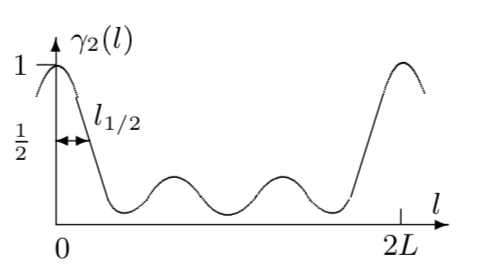
\includegraphics[scale=0.47]{v2.pdf}
	\caption{Измерение зависимости видности $ V_2 $ от дальности хода $ x $}
\end{figure}

\subsection{Измерение зависимости видности от дальности хода}


Теперь установим $ \alpha $ на максимальную видность и будем перемещать блок $ Б_2 $, тем самым изменяя дальность хода $ x $. Аналогично предыдущему пункту измерим величины $ h_1, h_2, h_3 \; и \; h_4 $ на экране осциллографа. Результаты занесем в таблицу и построим график согласно формуле \eqref{V2}. Значения для $ \delta, V, V_1 $ получим из формул выше.

\begin{table}[h!]
	\caption{Измерение зависимости видности от угла}
	\begin{center}
		\begin{tabular}{|c|c|c|c|c|c|c|c|c|}
			\hline
			$ 	\alpha  $ & $ h_4 $ &  $ h_3 $& $ h_2 $ & $ h_1 $ & $ V $ & $  \delta  $ & $ V_1 $ & $ V_2 $ \\
			\hline
		10 & 69 & 20 & 20 & 24 & 0.55 & 1.2 & 1 & 0.55 \\
		14 & 49 & 28 & 20 & 12 & 0.27 & 0.6 & 0.97 & 0.28 \\
		16 & 62 & 28 & 20 & 24 & 0.38 & 1.2 & 1 & 0.38 \\
		18 & 76 & 42 & 24 & 36 & 0.29 & 1.5 & 0.98 & 0.29 \\
		20 & 69 & 39 & 24 & 35 & 0.28 & 1.5 & 0.98 & 0.28 \\
		22 & 55 & 42 & 14 & 35 & 0.13 & 2.5 & 0.9 & 0.15 \\
		24 & 45 & 39 & 13 & 30 & 0.07 & 2.3 & 0.92 & 0.08 \\
		26 & 46 & 38 & 8 & 33 & 0.1 & 4.1 & 0.79 & 0.12 \\
		28 & 40 & 36 & 8 & 30 & 0.05 & 3.8 & 0.82 & 0.06 \\
		30 & 32 & 39 & 17 & 23 & -0.1 & 1.4 & 0.99 & 0.1 \\
		32 & 30 & 26 & 7 & 22 & 0.07 & 3.1 & 0.86 & 0.08 \\
		34 & 31 & 26 & 7 & 32 & 0.09 & 4.6 & 0.77 & 0.11 \\
		36 & 40 & 26 & 7 & 31 & 0.21 & 4.4 & 0.78 & 0.27 \\
		38 & 40 & 36 & 7 & 30 & 0.05 & 4.3 & 0.78 & 0.07 \\
		40 & 44 & 32 & 7 & 33 & 0.16 & 4.7 & 0.76 & 0.21 \\
		42 & 37 & 35 & 7 & 38 & 0.03 & 5.4 & 0.72 & 0.04 \\
		44 & 49 & 33 & 7 & 40 & 0.2 & 5.7 & 0.71 & 0.27 \\
		46 & 43 & 44 & 7 & 34 & -0.01 & 4.9 & 0.75 & 0.02 \\
		48 & 36 & 38 & 7 & 28 & -0.03 & 4 & 0.8 & 0.03 \\
		50 & 56 & 34 & 7 & 48 & 0.24 & 6.9 & 0.67 & 0.37 \\
		52 & 52 & 52 & 7 & 44 & 0 & 6.3 & 0.69 & 0 \\
		54 & 48 & 48 & 7 & 39 & 0 & 5.6 & 0.72 & 0 \\
		56 & 46 & 44 & 7 & 38 & 0.02 & 5.4 & 0.72 & 0.03 \\
		58 & 50 & 49 & 7 & 43 & 0.01 & 6.1 & 0.69 & 0.01 \\
		60 & 58 & 51 & 19 & 37 & 0.06 & 1.9 & 0.95 & 0.07 \\
		62 & 45 & 34 & 18 & 22 & 0.14 & 1.2 & 0.99 & 0.14 \\
		64 & 31 & 21 & 16 & 8 & 0.19 & 0.5 & 0.94 & 0.2 \\
		66 & 62 & 34 & 16 & 32 & 0.29 & 2 & 0.94 & 0.31 \\
		68 & 37 & 14 & 16 & 4 & 0.45 & 4 & 0.8 & 0.56 \\
		70 & 60 & 24 & 16 & 20 & 0.43 & 1.3 & 0.99 & 0.43 \\
		72 & 56 & 19 & 16 & 22 & 0.49 & 1.4 & 0.99 & 0.5 \\
		74 & 43 & 14 & 10 & 19 & 0.51 & 1.9 & 0.95 & 0.54 \\
		76 & 56 & 16 & 20 & 18 & 0.56 & 0.9 & 1 & 0.56 \\
		78 & 52 & 19 & 21 & 14 & 0.46 & 0.7 & 0.98 & 0.47 \\
		80 & 41 & 18 & 20 & 10 & 0.39 & 0.5 & 0.94 & 0.41 \\
			\hline
		\end{tabular}
	\end{center}
	\label{table_v2}
\end{table}

	Видно, что у нас наблюдается 2 максимума по краям области измерения и некоторые колебания в промежуточной области. А именно, максимумы в области $ x_1 \approx (10 \pm 2) \; см $ и в области $ x_2 \approx (75 \pm 2) \; см $, откуда получаем следующий результат:
	
	\begin{equation}\label{}
	L = \dfrac{1}{2} (x_2 - x_1) = (32,5 \pm 1,4) \; см
	\end{equation}
	
	Отсюда нетрудно получить и значение $ \Delta \nu $ из формулы \eqref{dnu}:
	
	\begin{equation}\label{}
	\Delta \nu = \dfrac{c}{2L} \approx (4,6 \pm 0,2) \x 10^8 \; Гц
	\end{equation}
	
	Оценим $ l_{1/2} \approx 18 - 10 = 8 \pm 2 $, откуда по формуле \eqref{dnu} получаем
	
\begin{equation}\label{}
  2\Delta F = 2\x \dfrac{0,26 c}{l_{1/2}} \approx (19,5 \pm 4,9) \x 10^8 Гц
\end{equation}

	Тогда для числа одновременно генерируемых лазером продольных волн можно провести оценку:
	
	\begin{equation}\label{}
	N \approx 1 + \dfrac{ 2\Delta F}{\Delta \nu} \approx 5 \pm 1
	\end{equation}
	



	
	\end{document}